%-------------------------------------------------------
\section{Validación del protocolo}
%-------------------------------------------------------
\subsection{Definición de Métricas}
\begin{frame}{Definición de Métricas}{Validación del protocolo}
%-------------------------------------------------------
\begin{block}{Métricas}
    \begin{enumerate}
    \justifying
        \item \textbf{Uso uniforme} del espacio de direccionamiento \textbf{(UU)}.\\ 
        \item \textbf{Latencia (LA)}: Retardo requerido para la asignación dinámica (setup initial y corrección de duplicidades) \cite{DATMANET}.\\
        {\tt t Latencia promedio por l -saltos\\
        d Diámetro de la red.}\\
        \item \textbf{Overhead (OV)}: Bytes requeridos para establecer el direccionamiento \cite{EvalSelf}\\
        {\tt n Número de dispositivos móviles.\\
        l Número de enlaces.\\
        p Payload.}
    \end{enumerate}
  \end{block}
\end{frame}
%-------------------------------------------------------
\subsection{Escenarios de Simulación}
\begin{frame}{Escenarios de Simulación}{Validación del protocolo}
%-------------------------------------------------------
% \begin{block}{Características escenarios de simulación en NS-3}
%  \begin{itemize}
%    \justifying
%    \item Cantidad aleatoria de nodos (entre 100 y 500), confinados en un espacio de dimensiones finitas.
%    \item La cantidad de recursos computacionales disponibles en cada nodo es asignada según un distribución normal.
%    \item Cada nodo estará dotado de una interfaz inalámbrica de bajo consumo energético. (Zigbee, 6LoWPAN, Wifi, LR-WPAN). 
%    \item Se otorgara movilidad 2D a un porcentaje variable nodos, empleando los modelos $"GaussMarkov2$ y $"Randomwaypoint"$.
%    \item El tráfico característico, es asignado bajo un modelo de $Poisson$. 
%    \item Mediante una distribución aleatoria uniforme, se seleccionan algunos nodos a los cuales se les 'apaga' la interfaz de comunicación.
%    \item Se iteran las simulacionespara identificar si la respuesta general del sistema es mejor debido al 'aprendizaje colectivo'.
%    \item Se somete DHCPv6 a los mismos escenarios.
%  \end{itemize}
% \end{block}
    \begin{figure}				
		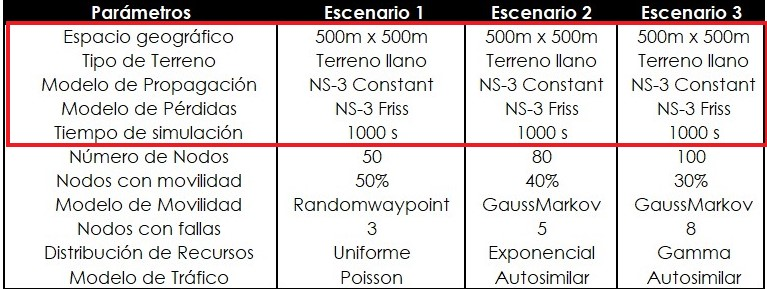
\includegraphics[width=\textwidth,height=\textheight,keepaspectratio]{Figures/ParSim.JPG}
		\caption{\small \sl Escenarios de simulación}
		\label{figure:ParSim}
    \end{figure}
\end{frame}
%-------------------------------------------------------
\begin{frame}{Escenarios de Simulación}{Validación del protocolo}
%-------------------------------------------------------
\begin{align}
RUNS &= l^{(k-p)}  \label{eqn5}\\
fractional_{n!} &= \frac{1}{l^{p}}  \label{eqn6}
\end{align}

Donde:\\
$l$ corresponde a los distintos niveles que puede asumir las variables.\\
$k$ el número de factores o variables estudiadas.\\
$p$ describe el tamaño de fracción del full factorial usado.\\

\begin{align*}
RUNS &= 3^{(6)} = 729  \\
RUNS &= 3^{(6-1)} = 243 => fractional_{n!} = \frac{1}{3^{1}}
\end{align*}
\end{frame}
%-------------------------------------------------------
%\begin{frame}{Escenarios de Simulación}{Validación del protocolo}
%-------------------------------------------------------
%    \begin{figure}				
%		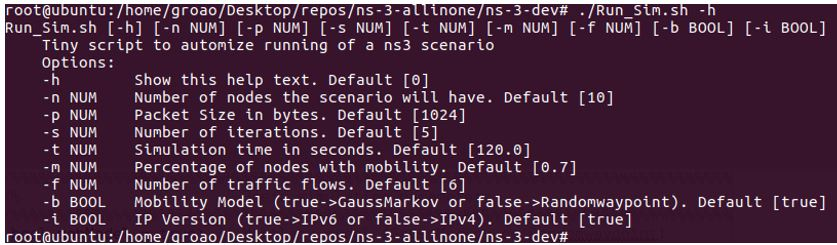
\includegraphics[width=1.\textwidth,height=1.\textheight,keepaspectratio]{Figures/Bash.JPG}
%		\caption{\small \sl Bash script}
%		\label{figure:Bash}
    %\end{figure}
    %\begin{figure}				
%		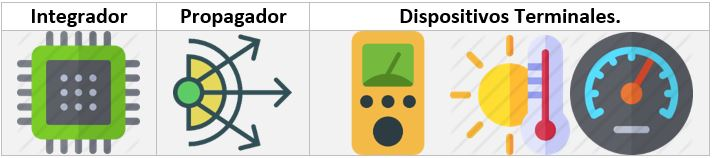
\includegraphics[width=0.8\textwidth,height=0.8\textheight,keepaspectratio]{Figures/Devices.JPG}
%		\caption{\small \sl Devices}
%		\label{figure:Devices}
%    \end{figure}
%\end{frame}
%-------------------------------------------------------
\begin{frame}{Escenarios de Simulación}{Validación del protocolo}
%-------------------------------------------------------
	\centering
	\begin{figure}
	%\includemedia[
	    %label=myVidPlayer,
        %width=10cm,height=10cm,
        %activate=pageopen,
    %    addresource=Figures/Avance.mp4,
    %    flashvars={
    %    source=Figures/Avance.mp4
    %    &autoPlay=true
    %    &loop=true
        %&scaleMode=letterbox
    %    },
    %    passcontext
    %]{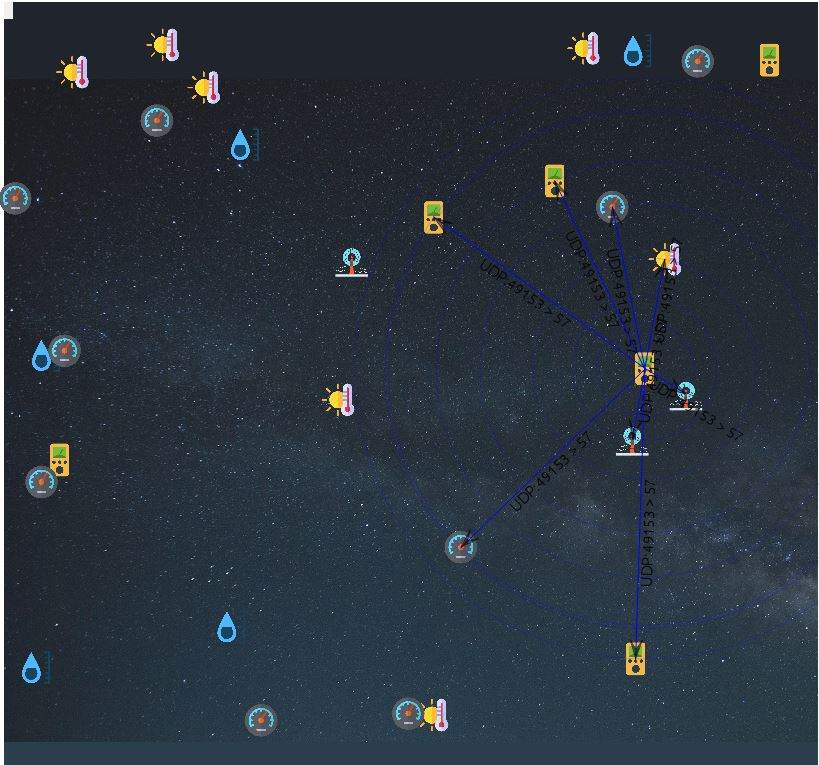
\includegraphics[width=0.8\textwidth,height=0.75\textheight,keepaspectratio]{Figures/Sim.JPG}}{VPlayer9.swf}
    {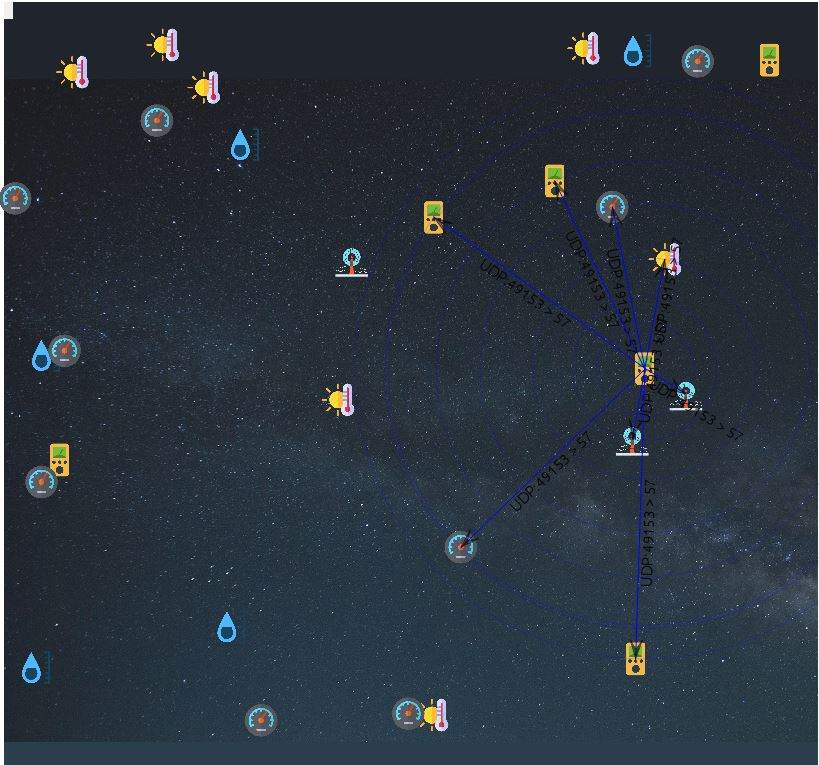
\includegraphics[height=0.75\textheight,keepaspectratio]{Figures/Sim.JPG}}
    \caption{\small \sl Ejemplo Simulación}
	\label{figure:EjemploSim}
	\end{figure}
%-------------------------------------------------------
\end{frame}
%-------------------------------------------------------
\subsection{Resultados}
\begin{frame}{Resultados}{}
%-------------------------------------------------------
    \begin{itemize}
    \justifying
    \item<1-|alert@1> \centering 
\includegraphics[width=0.4\textwidth,height=0.3\textheight,keepaspectratio]{Figures/Tableau.JPG}
    \item<2-|alert@2> Se debe reformular la ecuación (3) \begin{align} Max(\# Devices) &= \left[ AS_{propagator}*AS_{integrator}* \gamma \right ]  \label{eqn7}
\end{align} Donde $\gamma$ corresponde a un factor de seguridad de diseño. Experimentalmente se corroboró que un valor aceptable debe ser máximo \textbf{0.6}.
    \item<3-|alert@3> Se reformula la ecuación (4) \begin{equation}
    %\centering
    Min Propagator(n)=\left\{ \begin{array}{ccc}
            \frac{r+a+d}{D(n)} & n \leq 50 \\
            \\
            \frac{\# Terminals}{AS_{propagator}} + D(n)(r+a+d) & n > 50 
             \end{array}
   \right. \label{eqn8}
    \end{equation}  
  \end{itemize}
\end{frame}
%-------------------------------------------------------